\chapter{Fonction sinus et cosinus}
\thispagestyle{fancy}

\vspace{-0.5cm}

	\section{Résoudre une équation trigonométrique}
	
		\begin{bmethodet}{Résoudre une équation trigonométrique}
			\grasInMet{Enoncé :}\\
			Résoudre sur $[3\pi;5\pi]$ l'équation $\cos x=\dfrac{\sqrt{3}}{2}$
			\grasInMet{Réponse :}\\
			\ \\
			\begin{minipage}{0.65\linewidth}
				On commence par étudier la solution dans l'intervalle\\ $]-\pi;\pi]$ (parmi les mesures principales de l'angle).\\
				L'équation $\cos x=\dfrac{\sqrt{3}}{2}$ a pour solution :\\
				$\begin{cases}
					x_1 &=\dfrac{\pi}{6}\\
					x_2 &=-\dfrac{\pi}{6}
					\end{cases}$\\
				On en déduit les solutions sur \R.\\
				L'équation $\cos x=\dfrac{\sqrt{3}}{2}$ a pour solution ($k\in \Z$ ) :\\
				$\begin{cases}
						x_1 &=\dfrac{\pi}{6}+2k\pi\\
						x_2 &=-\dfrac{\pi}{6}+2k\pi\
					\end{cases}$\\
				On teste différentes valeurs de $k$ pour trouver les valeurs qui appartiennent à l'intervalle souhaité $[3\pi;5\pi]$ (ou $\left[\dfrac{18\pi}{12};\dfrac{30\pi}{6}\right]$)\\
				$k=1\quad \begin{cases}
						x_1 &=\dfrac{\pi}{6}+2\pi=\dfrac{13\pi}{6}\notin\left[\dfrac{18\pi}{12};\dfrac{30\pi}{6}\right]\\
						x_2 &=-\dfrac{\pi}{6}+2\pi=\dfrac{11\pi}{6}\notin\left[\dfrac{18\pi}{12};\dfrac{30\pi}{6}\right]
					\end{cases}$\\
				$k=2\quad \begin{cases}
						x_1 &=\dfrac{\pi}{6}+4\pi=\dfrac{25\pi}{6}\in\left[\dfrac{18\pi}{12};\dfrac{30\pi}{6}\right]\\
						x_2 &=-\dfrac{\pi}{6}+4\pi=\dfrac{23\pi}{6}\in\left[\dfrac{18\pi}{12};\dfrac{30\pi}{6}\right]
					\end{cases}$\\
				$k=3\quad \begin{cases}
						x_1 &=\dfrac{\pi}{6}+6\pi=\dfrac{37\pi}{6}\notin\left[\dfrac{18\pi}{12};\dfrac{30\pi}{6}\right]\\
						x_2 &=-\dfrac{\pi}{6}+6\pi=\dfrac{35\pi}{6}\notin\left[\dfrac{18\pi}{12};\dfrac{30\pi}{6}\right]
					\end{cases}$\\
				On peut maintenant conclure : $S=\left\{\dfrac{23\pi}{6};\dfrac{25\pi}{6}\right\}$
				\end{minipage} \hfill
				\begin{minipage}{0.35\linewidth}
					\begin{center}
							\includegraphics[scale=0.35]{01-02-16}
						\end{center}
				\end{minipage}
				
			\end{bmethodet}

%     \section{Représentations graphiques}
%     \begin{center}
%         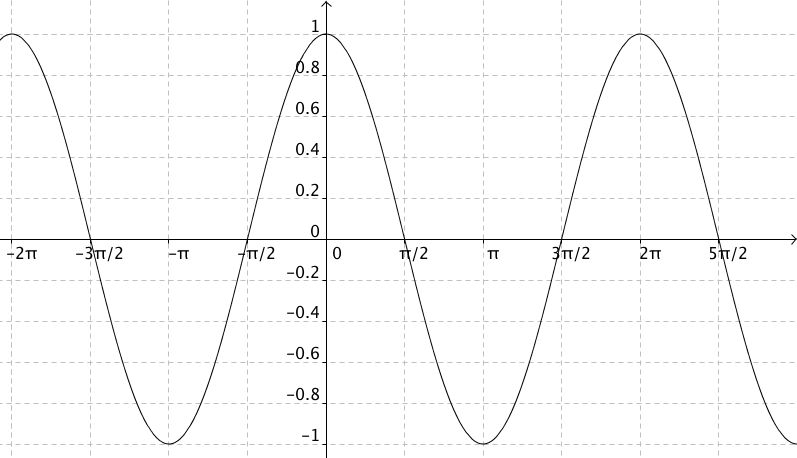
\includegraphics[scale=0.4]{../images/01-02-18.png}\\
%         Fonction cosinus
%     \end{center}
%     \begin{center}
%         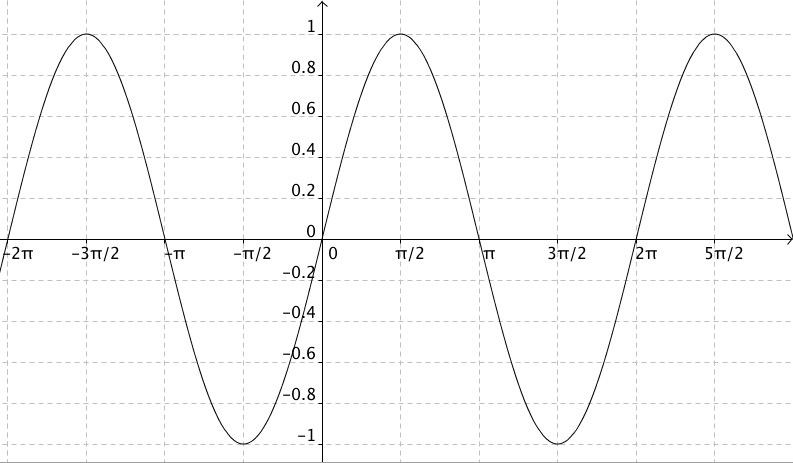
\includegraphics[scale=0.4]{../images/01-02-19.png}\\
%         Fonction sinus
%     \end{center}
%    
%     \section{Périodicité}
%    
%     On a vu que :  $\cos x=\cos(x+2k\pi)$ où $k$ entier relatif et  $\sin x=\sin(x+2k\pi)$ où $k$ entier relatif.
%    
%     \begin{bprop}
%         On dit que les fonctions cosinus et sinus sont \grasInDef{périodiques de période $2\pi$}.
%     \end{bprop}
%    
%     \begin{bcscq}
%         Pour tracer la courbe représentative de la fonction cosinus ou de la fonction sinus, il suffit de la tracer sur un intervalle de longueur $2\pi$ et de la compléter par translation.
%     \end{bcscq}
%    
%     \section{Parité}
%    
%     On a vu que :  $\cos(-x)=\cos(x)$ et  $\sin(-x)=-\sin x$.
%    
%     \begin{bprop}
%         On dit que la fonctions \grasInDef{cosinus est paire} et que la fonction \grasInDef{sinus est impaire}.
%     \end{bprop}
%    
%     \begin{bcscq}
%         - Dans un repère orthogonal, la courbe représentative de la fonction cosinus est symétrique par rapport à l'axe des ordonnées.\\
%         - Dans un repère orthogonal, la courbe représentative de la fonction sinus est symétrique par rapport à l'origine.
%     \end{bcscq}
%    
%     \section{Variations des fonctions cosinus et sinus}
%    
%         \begin{multicols}{2}
%             \begin{tikzpicture}
%                 \tkzTabInit{$x$ / 1 , $\sin(x)$ / 1.5}{$0$, $\dfrac{\pi}{2}$, $\pi$}
%                 \tkzTabVar{-/ 0, +/ 1, -/ 0}
%             \end{tikzpicture}
%            
%             \begin{tikzpicture}
%                 \tkzTabInit{$x$ /1, $\cos(x)$ /1.5} {$0$ , $\pi$}
%                 \tkzTabVar{+/ 1, -/ -1}
%             \end{tikzpicture}
%         \end{multicols}
     
%     \section{Fonctions cosinus et sinus}
     
     \section{Définitions et représentations graphiques}
     \begin{bdefis}
     	\begin{itemDef}
     		\item La fonction cosinus est la fonction définie sur $\mathbb{R}$ qui, à tout réel $x$, associe $\cos (x)$.
     		\item La fonction sinus, est la fonction définie sur $\mathbb{R}$ qui, à tout réel $x$, associe $\sin (x)$.
     	\end{itemDef}
     
     	
     \end{bdefis}
 
 	\begin{minipage}[c]{0.45\linewidth}
 		\begin{center}
 			\includegraphics[scale=0.15]{2024_01_04_295cf56f03985ebac5b3g-06(1)}
 		\end{center}
 		
 		Fonction cosinus
 	\end{minipage} \hfill
 	\begin{minipage}[c]{0.45\linewidth}
 		\begin{center}
 			\includegraphics[scale=0.15]{2024_01_04_295cf56f03985ebac5b3g-06}
 		\end{center}
 		
 		Fonction sinus
 	\end{minipage}
     
     
     
     
     
     \section{Périodicité}
     
     \begin{bprops}
     	\begin{itemProp}
     		\item $\cos (x)=\cos (x+2 k \pi)$ où $k$ entier relatif.
     		\item $\sin (x)=\sin (x+2 k \pi)$ où $k$ entier relatif.
     	\end{itemProp}
     \end{bprops}
     
     \begin{bdemo}
     	Aux points de la droite orientée d'abscisses $x$ et $x+2 k \pi$ ont fait correspondre le même point du cercle trigonométrique.
     \end{bdemo}
 
 	\begin{brmq}
 		On dit que les fonctions cosinus et sinus sont périodiques de période $2 \pi$.
 		
 		Cela signifie qu'on retrouve le même morceau de courbe sur chaque intervalle de longueur $2 \pi$.
 	\end{brmq}
     
     \subsection{Fonction cosinus}
     \begin{center}
     	\includegraphics[scale=0.2]{2024_01_04_295cf56f03985ebac5b3g-07(2)}
     \end{center}
     
    
     \subsection{ Fonction sinus}
     \begin{center}
     	\includegraphics[scale=0.2]{2024_01_04_295cf56f03985ebac5b3g-07(1)}
     \end{center}
 
 	\section{Parité}
     
     \begin{bdefis}
     	\begin{itemDef}
     		\item Une fonction dont la courbe est symétrique par rapport à l'axe des ordonnées est une fonction paire.
     		\item Une fonction dont la courbe est symétrique par rapport à l'origine du repère est une fonction impaire.
     	\end{itemDef}	
     \end{bdefis}
     	
     
    \begin{brmqs}
    	\begin{itemRem}
    		\item Pour une fonction paire, on a : $f(-x)=f(x)$.
    		\item Pour une fonction impaire, on a : $f(-x)=-f(x)$.
    	\end{itemRem}
    	Ce sont ces résultats qu'il faudra vérifier pour prouver qu'une fonction est paire ou impaire.	
    \end{brmqs}
    
     
     
     \begin{bprops}
     	\begin{itemProp}
     		\item La fonction cosinus est paire et on a : $\cos (-x)=\cos (x)$
     		\item La fonction sinus est impaire et on a : $\sin (-x)=-\sin (x)$
     	\end{itemProp}	
     \end{bprops}
     
     \begin{bdemo}
     	Les angles de mesures $x$ et $-x$ sont symétriques par rapport à l'axe des abscisses donc :
     	
     	$\sin (-x)=-\sin x$ et $\cos (-x)=\cos x$.
     	
     	\begin{center}
     		\includegraphics[scale=0.2]{2024_01_04_295cf56f03985ebac5b3g-07}
     	\end{center}
     \end{bdemo}
     
     \begin{brmqs}
     	\begin{itemRem}
     		\item La courbe de la fonction cosinus est symétrique par rapport à l'axe des ordonnées.
     		\item La courbe de la fonction sinus est symétrique par rapport à l'origine.
     	\end{itemRem}
     \end{brmqs}
 
 	\section{Méthodes}
     
     \begin{bmethodet}{Reconnaître graphiquement la parité et la périodicité d'une fonction}
     	\grasInMet{Enoncé:}\\
     	Déterminer graphiquement la parité et la périodicité des fonctions $f, g$ et $h$ représentées ci-dessous :
     	\begin{center}
     		\includegraphics[scale=0.2]{2024_01_04_295cf56f03985ebac5b3g-08}
     	\end{center}
     	\grasInMet{Corrigé:}\\
     	\grasInMet{- FONCTION $\boldsymbol{f}$ :}\\
     	La fonction $f$ est paire car sa courbe est symétrique par rapport à l'axe des ordonnées.
     	\begin{center}
     		\includegraphics[scale=0.15]{2024_01_04_295cf56f03985ebac5b3g-09(2)}
     	\end{center}
     	La fonction $f$ est périodique de période $\pi$ car on retrouve le même morceau de courbe sur chaque intervalle de longueur $\pi$.
     	\begin{center}
     		\includegraphics[scale=0.15]{2024_01_04_295cf56f03985ebac5b3g-09(3)}
     	\end{center}
     	\grasInMet{- FONCTION $g$ :}\\
     	La fonction $g$ est impaire car sa courbe est symétrique par rapport à l'origine.
     	\begin{center}
     		\includegraphics[scale=0.15]{2024_01_04_295cf56f03985ebac5b3g-09(1)}
     	\end{center}
     	La fonction $g$ est périodique de période $\frac{\pi}{2}$ car on retrouve le même morceau de courbe sur chaque intervalle de longueur $\frac{\pi}{2}$.
     	\begin{center}
     		\includegraphics[scale=0.15]{2024_01_04_295cf56f03985ebac5b3g-09}
     	\end{center}
     	\grasInMet{- FONCTION $h$ :}\\
     	La fonction $h$ est paire car sa courbe est symétrique par rapport à l'axe des ordonnées.
     	\begin{center}
     		\includegraphics[scale=0.15]{2024_01_04_295cf56f03985ebac5b3g-10(1)}
     	\end{center}
     	La fonction $h$ n'est pas périodique, on ne retrouve pas le même morceau de courbe sur différents intervalles.
    \end{bmethodet}

	\begin{bmethodet}{Étudier la parité d'une fonction trigonométrique}
		\grasInMet{Enoncé:}\\
		Démontrer que la fonction $f$ définie sur $\mathbb{R} \operatorname{par} f(x)=\sin (x)-\sin (2 x)$ est impaire.\\
		\grasInMet{Corrigé:}\\
		On a :
		
		$f(-x)=\sin (-x)-\sin (-2 x)=-\sin (x)+\sin (2 x)=-(\sin (x)-\sin (2 x))=-f(x)$. La fonction $f$ est donc impaire.
		
		Sa représentation graphique est symétrique par rapport à l'origine du repère.
	\end{bmethodet}

	\begin{bmethodet}{Compléter un graphique par parité et périodicité}
		\grasInMet{Enoncé:}\\
		Soit $f$ une fonction impaire et périodique de période $\pi$. Compléter sa représentation graphique sur l'intervalle $\left[-\frac{3 \pi}{2} ; \frac{3 \pi}{2}\right]$.
		
		\begin{center}
			\includegraphics[scale=0.2]{2024_01_04_295cf56f03985ebac5b3g-10}
		\end{center}
		\grasInMet{Corrigé:}\\
		$1^{\text {ère }}$ étape : La fonction est impaire. Sa courbe représentative est symétrique par rapport à l'origine du repère.
		
		On complète donc par symétrie centrale.
		
		\begin{center}
			\includegraphics[scale=0.2]{2024_01_04_295cf56f03985ebac5b3g-11(1)}
		\end{center}
		
		$2^{\mathrm{e}}$ étape : La fonction est périodique de période $\pi$. On retrouve le même morceau de courbe sur chaque intervalle de longueur $\pi$.
		
		Le morceau déjà tracé a pour longueur $\pi$, on le reproduit à gauche et à droite.
		
		\begin{center}
			\includegraphics[scale=0.2]{2024_01_04_295cf56f03985ebac5b3g-11}
		\end{center}
	\end{bmethodet}

